\scanpage{5}
% Archive foliation: 4, lower left.
\unsure{i)|h)} Possibilité de définir \unsure{des|un} invariants
$K(\mathcal H)$ via ``triangles exacts'', voire $K_n$
supérieurs d'une théorie homotopique.
\margin{(Cas additif seulement ?!?)}
\margin{\figure{\begin{tikzpicture}[scale=.5]\draw[<->] (0,3)--(1.2,0);\end{tikzpicture}}}

\deleted{\unsure{j)}}\inserted{h)} Souvent il y a \inserted{des} $\uline{\operatorname{Hom}}$ internes
dans $\mathcal H$, avec \deleted{\unsure{des}}\inserted{une} formule du type
\[
\operatorname{Hom}(\unsure{f|\xi},\unsure{g|\eta})
=\Gamma\,\uline{\operatorname{Hom}}(\unsure{f|\xi},\unsure{g|\eta})\unsure{)|\}}
\]
\margin{Structure multiplicative et structure $\operatorname{Hom}$}
\[
\Gamma\text{ ou }\pi_0:\mathcal H\longrightarrow\mathrm{Ens}
\]
un foncteur \unsure{important|imposé} (souvent
$\operatorname{Hom}(1,-)$, où $1$ un objet unité\ldots)
\margin{(24.11.83) Relations entre ces $\uline{\operatorname{Hom}}$ internes et les
$\uline{\operatorname{Homhot}}(x,y)\in\operatorname{Ob}\mathrm{Hot}$
dans e) ??}

Souvent aussi, Structure multiplicative
(soit produit cartésien, soit un produit $\otimes$)
avec une formule
\[
\operatorname{Hom}(x\otimes y,z)\simeq
\operatorname{Hom}(x,\uline{\operatorname{Hom}}(y,z))
\]
\figure{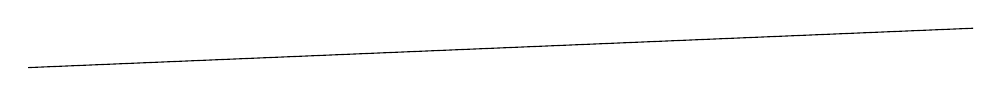
\begin{tikzpicture}\draw (0,0)--(12,.5);\end{tikzpicture}}
Sauf peut-être les Structures
f) et g), il semble que tout puisse
se décrire en termes de $(M,W\subset\operatorname{Fl}(M))$.
\uline{Dégager les bons axiomes}
